% !eX root = ../tfm.tex
%! TEX root = ../tfm.tex

Tras un primer contacto con los componentes escogidos para implementar la aplicación \accelcapture/ en el capítulo anterior nos enfrentamos al desarrollo de la plataforma final. Empezaremos recuperando la base de datos \sisfall/  como mencionamos en el capítulo de requisitos (Sección \ref{sec:req:bases:datos}) para implementar un prototipo del algoritmo, lo describiremos, analizaremos los resultados y compararemos con otros métodos ya existentes. Con el modelo validado nos centraremos en optimizarlo para mejorar el consumo de recursos de cara al siguiente paso: implementar la aplicación y sistema final. Explicaremos la estructura del sistema cliente-servidor escogida y entraremos en detalle en el estudio y análisis de la aplicación para dispositivos llevables presentada. Estudiaremos la arquitectura, interfaz de uso y rendimiento antes de abordar, en el capítulo siguiente la idoneidad y adecuación a los requisitos previamente definidos 

\section{Descripción de la base de datos}

Para la primera etapa de generación y evaluación del algoritmo y modelos analíticos y RNN hemos elegido el conjunto de datos \sisfall/. El conjunto de bases de datos libres para la detección de caídas es todavía muy reducido, muchas veces estos conjuntos de datos están demasiado centrados en maximizar el rendimiento del modelo para el que fueron creados. En el estudio realizado por \citeA{igual2015} analiza entre otros \textit{MobiFall} \cite{MobiFall} y \textit{tFall} \cite{tfall}. Estudia el impacto en los resultados de usar cada conjunto para el entrenamiento y validación y posteriormente la capacidad de generalizar o de crear mejores modelos de cada uno de ellos, llegando a la misma conclusión: los conjuntos de datos existentes hoy en día están demasiado enfocados a un experimento concreto y por tanto recomienda normalizar y usar varios de ellos. En el mismo estudio se recomienda encarecidamente usar más de una base de datos para el entrenamiento y validación para sobrellevar esta limitación. Un segundo resultado de interés es que \textquote[{\citeNP[p.~15]{igual2015}}]{muestrear a 100\hz/ no es mejor que hacerlo a 50\hz/} que confirma estudios previos indicando que hasta 25\hz/ podrían ser suficientes, ya que esta será la frecuencia de muestreo usada en nuestra aplicación.


\begin{table}[ht]
% \tablas{tab:id}{Título tabla}{lcccl}{ la tabla propiamente dicha }
  \subtablal[0.4]{tab:sisfall:population}{Edad, y peso de los sujetos}{lcc}{
    \textsl{Grupo}  & \textsl{Edad}  & \textsl{Peso (kg)} \\\midrule
    Adultos & 60-75 & 50 - 102 \\
    Jóvenes & 19-30 & 42 - 81 \\
}{2}%
\hfill
\subtablar[0.4]{tab:sisfall:tecnicos}{Características de las medidas}{lr}{
\textit{Característica}  & \textit{Valor} \\ \midrule
Muestreo                & 200\hz/ \\
Rango                   & $\pm$ 16\g/\\
Precisión               & 16 bits \\
Componentes             & 3 ejes \\
}{2}


\subtablac[0.6]{tab:sisfall:caracteristicas}{Especificaciones de la base de datos \sisfall/}{lrl}{
\textit{Característica} & \textit{Valor} & \textit{Notas} \\ \midrule
Participantes           & 38            &  15 jóvenes y 23 personas mayores. \\
Clases de eventos       & 34            &  \\
Tipos de Caídas         & 15            &  Todas las caídas son simuladas.\\
Tipos de Actividades    & 19            &  \\
Total de eventos        & 4504          &  \\
de las cuales Caídas    & 1798          &  El 40\% de eventos.Claramente sobrerrepresentadas  \\
de las cuales Actividades & 2706        &  \\
}{2}

\caption{\label{tab:sisfall:tablas} Características y tratamiento de la base de datos \sisfall/}
\end{table}

Estudiando las características de los conjuntos de datos, finalmente optamos por \sisfall/ \cite{Sucerquia2017}. Este conjunto está altamente centrado en la detección de caídas en personas mayores. En el análisis de los resultados obtenidos se sugiere de nuevo que \textquote[{\citeNP[p.~9]{Sucerquia2017}}]{frecuencias de muestreo de tan solo 11\hz/ podrían ser suficientes para la detección de caídas}, dado que el estimador que mejor funciona es el módulo del vector aceleración. Destaca el tamaño de la base de datos, la presencia de personas de edad avanzada entre los sujetos de estudio y el énfasis en la detección de caídas, con una clara abundancia de caídas (casí un 40\% del total de eventos) así como la presencia de eventos similares a caídas entre las actividades cotidianas (saltar, sentarse rápidamente, tropezar, caer en una silla al intentar levantarse y otras, totalizando hasta 8 de las 19 categorías de actividad) que suponen el peor escenario al que podemos someter un clasificador. Como afirma el propio estudio y verificaremos en este, usar un conjunto de datos tan centrado en la detección de caídas resultará un reto añadido para el clasificador a desarrollar.

Resumimos en las tablas \ref{tab:sisfall:tablas} las principales características de \sisfall/, aunque recomendamos visitar \url{https://github.com/WJMatthew/SisFallAnalysis} por contener un estupendo análisis del mismo con gran variedad de gráficos explicativos.

\subsection{Preprocesado de la base de datos}

Con el fin de reducir el número de eventos producidos, y partiendo de la premisa de que con un ancho de banda de 12\hz/ en la señal módulo de la aceleración hay suficiente información para realizar la detección de caídas \cite{Liu2018}, submuestrearemos el conjunto de datos \sisfall/ desde los 200\hz/ originales a 25\hz/. Dado que esta será la frecuencia de lectura que usará el dispositivo final, permitirá obtener una evaluación del rendimiento en similares condiciones.

\paragraph{Filtrado IIR}

Previo al subsampleado de la señal optamos por realizar un filtrado paso bajo respecto a la frecuencia de corte de Nyquist para señales muestreadas a 25\hz/ ($f_c=\frac{25}{2}=12,5$). Usaremos un filtro IIR de primer orden, con función de transferencia $H(z)$:

\[
  y_n = \alpha x_n + (1-\alpha) y_{n-1}
\]

%comment = \alpha\times x_n + \(1-\alpha\)\times y_{n-1}

\[
  H(z) = \frac{\alpha}{1-(1-\alpha)z^{-1}}
\]

Donde
\begin{align*}
\alpha = \frac{\delta t}{\delta t + RC} \\
f_c= \frac{1}{2 \pi RC}
\end{align*}

Como posteriormente submuestrearemos la señal a 25\hz/ y que sabemos que en estos primeros 12\hz/ hay suficiente información sobre las caídas, tomamos como ya hemos dicho $f_c=12,5Hz$. Hay que tener en cuenta que al ser un filtro paso bajo no afectará a la componente continua de la gravedad, lo cual es necesario para poder utilizar el modelo Bourke. Despejando las ecuación precedentes queda:
\begin{align*}
  f_m & = 200{Hz}\\
  \delta t & = 1/f_m = 0.005s\\
  RC & =\frac{1}{2\pi f_c} = \frac{1}{2\pi12,5} = 0,5\\
  \alpha & = \frac{0.02}{0.02 + RC} = 0,015
\end{align*}

\iffalse
%VER https://electronics.stackexchange.com/questions/498226/calculate-cutoff-frequency-of-a-digital-iir-filter
%https://en.wikipedia.org/wiki/EWMA_chart
%https://en.wikipedia.org/wiki/Low-pass_filter#Simple_infinite_impulse_response_filter
\fi

El interés de realizar un filtrado previo al subsampleado puede observarse al compararse los resultados expuestos en la figura \ref{fig:iir} en ella se observa la destrucción de información producida por el muestreado de la señal. Se aprecia claramente como en las curvas de la figura\ref{fig:signalIIRFilter25} en que se ha muestreado la señal sin filtrado previo se ha aplanado en exceso. Resultado especialmente nocivo para nuestro modelo analítico que se basa precisamente en detectar estos picos valles. En el propio trabajo de \citeauthorNP{Sucerquia2017} se recomienda usar un filtrado ya que según sus resultados en promedio mejora la capacidad de detección de los modelos entrenados y otros estudios \cite{Xiao2016,Tian2019,Liu2020} demuestran la efectividad de un filtrado previo de los conjuntos de entrenamiento para mejorar la precisión de los modelos.

\begin{figure}[htb!]
  \centering
  \begin{subfigure}[b]{0.96\textwidth}
      \centering
      \pincludegraphics[0.9]{FilterAndDownsample}
      \caption{\footnotesize Degradación de la señal con submuestreados y filtrados}
      \label{fig:downsample}
  \end{subfigure}
  \centering

  \begin{subfigure}[b]{0.48\textwidth}
      \centering
      \pincludegraphics[1.0]{SignalvsIIRFilter}
      \caption{\footnotesize Señal original (200Hz) y filtrada}
      \label{fig:signalIIRFilter}
  \end{subfigure}
  \hfill
  \begin{subfigure}[b]{0.48\textwidth}
      \centering
      \pincludegraphics[1.0]{SignalvsIIRFilter25Hz}
      \caption{\footnotesize Señal submuestreada a 25\hz/ y filtrada}
      \label{fig:signalIIRFilter25}
  \end{subfigure}
  \caption{\footnotesize \label{fig:iir}  Efecto del filtro IIR y submuestreado en la señal}
\end{figure}

\paragraph{Submuestreado a 25\hz/}

La base de datos \sisfall/ usa un muestreado a 200\hz/, el reloj elegido como soporte admite únicamente un muestreado a 50\hz/ como máximo. Sin embargo reduciremos la frecuencia de lectura a 25\hz/ para reducir el número de cáclulos a realizar ya que los experimentos previos demuestran que es posible detectar caídas incluso con 11\hz/. El sub-muestreado se realiza tomando una muestra de cada n con $n=\frac{f_m}{f_o}=\frac{25}{200}=8$. En la figura \ref{fig:downsample} se aprecia la degradación que sufre la señal original al aplicarle el filtrado y posterior reducción de muestras. Se observa un doble efecto del filtrado: un suavizado de la señal resultante y un desfase no lineal. El suavizado enmascara parcialmente los valores pico y valle, sin embargo garantiza mayor fidelidad del resultado a la señal original: si bien se pierde la información en picos y valles, la señal mantiene mejor la estructura general. En el fondo se ha reducido el ruido de la señal ya que el filtro en la práctica actúa como un ponderador.


\section{Descripción del Modelo y Algoritmo de \ifell/}\label{sec:imp:model}

Se ha mencionado ya en varios momento que el uso de un dispositivo de medida de la aceleración en la muñeca no resulta idóneo para realizar predicciones sobre la realización de actividades o caídas. Este será el principal escollo al que deberá hacer frente el algoritmo elegido ya que no afectará únicamente a la viabilidad de las medidas. La misma razón que afecta negativamente a la capacidad predictora de las mediciones en la muñeca, la excesiva movilidad de las extremidades, tiene un segundo efecto espúreo: al tener mayor libertad de movimiento, también se generan más eventos de actividad incluso cuando el sujeto se encuentra en reposo. Valga de ejemplo el hecho de que mirar la hora es suficiente para activar el detector de actividad de \accelcapture/ (\autoref{sub:accelcapture:flujo}) mientras que con cualquier otro emplazamiento del sensor no habría habido lectura alguna. Debemos encontrar una solución que permita reducir el número de veces que evaluamos si se ha producido una caída para reducir el consumo del sistema y dotarlo de mayor autonomía.

\subsection{Algoritmo híbrido}\label{sub:imp:model:algoritmo}

Buscando encontrar un equilibrio entre capacidad de detección y requisitos del sistema, optamos por un algoritmo híbrido con dos modelos (uno analítico y otro basado en redes recurrentes), tal y como se presenta en la \autoref{fig:ifell:algoritmo}. Al utilizar dos etapas permite mantener el costoso modelo neuronal aletargado a la espera de un evento del modelo analítico. Este modelo, más simple, apenas consiste de un comparador, puede ejecutarse sin problema de forma continua sin tener un impacto notable en la duración de la batería del sistema\todo{referencia a la gráfica de consumos de batería}. 

\figura[0.5]{deteccionFlujo}{fig:ifell:algoritmo}{Algoritmo de detección de caídas de \ifell/}

Si analizamos el algoritmo, apreciamos su similitud con el de la aplicación de captura de datos. En parte por el hecho de que la primera etapa es idéntica: Un sistema generador de eventos cuando se detecta actividad. En este caso este primer sistema generador de eventos es el modelo analítico. El acelerómetro del sistema genera lecturas de los tres ejes de la aceleración a un ratio determinado (25 muestras por segundo). Estas muestras se convierten en el módulo de la aceleración $\|\vec{A}\|=\sqrt{A_x^2 + A_y^2 + A_z^2}$ y se almacenan en una cola de 4 segundos o 100 muestras. Tras cada lectura de una nueva muestra, el modelo analítico elegido procesa su contenido y genera un evento de caída si así lo detecta. De ser así, se envía el contenido de la cola al modelo neuronal que discriminará si efectivamente es una caída o no.

El modelo analítico o generador de eventos usado es un comparador de Bourke, que definiremos en el siguiente punto. El detector basado en redes neuronales a usar puede ser tanto un modelo basado en el error de reconstrucción, o un modelo basado en el error de predicción. Como veremos en la sección \fullref{sub:imp:model:rnn} estudiaremos ambos modelos para dilucidar cual se ajusta mejor a los requisitos formulados ya que aunque muy similares en estructura y funcionamiento, tanto la precisión como latencia del modelo varía sensiblemente entre ambos.

\subsection{Modelo Analítico: Bourke}\label{sub:imp:model:analitico}

Justificamos ya en la \autoref{sec:req:modelos} la necesidad de usar modelos que no analicen la postura, posición o inclinación del sensor debido a la falta de coherencia entre la posición del sensor respecto la del cuerpo por su situación en la muñeca. Este factor, que tendrá un impacto en la calidad del modelo obtenido infiere a la vez de mayor simplicidad y facilitará su posterior uso en sistemas embebidos por su bajo consumo de recursos.

Elegimos usar un clasificador de Bourke. Presentado por \citeA{Bourke2006} es un algoritmo simple que al no requerir más que del módulo del vector aceleración cumple con los requisitos para ser usado en nuestro sistema (principalmente no requerir de información inercial ni postural, únicamente el módulo de la aceleración). Usando dos cotas de detección consecutivas (una cota inferior para detectar valles en la aceleración y una superior para la detección del posterior pico como se muestra en la \autoref{fig:bourke_thresholds}) permite identificar caídas basándose en la forma característica que sigue la aceleración del cuerpo en estos eventos. Tradicionalmente se estudian dos variantes adicionales de este clasificador que consisten en modelos que analizan cuando se dan por separado cada una de las condiciones. Al modelo principal que mide las cuotas de pico y valle lo designaremos \textit{BourkeUL}, y \textit{BourkeU} y \textit{BourkeL} a los modelos que estudian únicamente las cotas de pico o valle respectivamente. Estudiaremos el comportamiento de cada variante con la esperanza de poder justificar el uso de una de las variantes parciales por su mayor simplicidad.

Como el resto de modelos analíticos aplicados a la detección de caídas tiene la gran ventaja de ser computacionalmente simple. Su mayor contraprestación es la dificultad de balancear las métricas de Especificidad y Sensibilidad. Al basarse en niveles o cotas, podemos aumentar la sensibilidad situando el nivel de estas de manera que la sensibilidad llegue al 100\%, como requiere el algoritmo por definición, aunque afectará a la especificidad negativamente \cite{Aziz2017} pues cuanto más ajustemos estos niveles de decisión más probable es que incluyamos casos de actividades cotidianas dentro del rango de caídas. Este solapamiento lo podremos estudiar al analizar las densidades de probabilidad e histogramas de los valores para actividades y caídas, como en la \autoref{fig:bourke:hist}.

\begin{figure}[htb!]
  \centering
  \begin{subfigure}[b]{0.48\textwidth}
      \centering
      \pincludegraphics[1.1]{BourkeLowThresholdsHistogram}
      \caption{\footnotesize Histograma valores \textit{valle} modelo Bourke}
      \label{fig:bourke:hist:low}
  \end{subfigure}
  \hfill
  \begin{subfigure}[b]{0.48\textwidth}
      \centering
      \pincludegraphics[1.1]{BourkeUpperThresholdsHistogram}
      \caption{\footnotesize Histograma valores \textit{pico} modelo Bourke}
      \label{fig:bourke:hist:high}
  \end{subfigure}
  \caption{\label{fig:bourke:hist} Histogramas de valores pico y valle}
\end{figure}

En nuestro algoritmo general, el modelo analítico es similar a una capa de gestión de la atención del modelo RNN. Es por esta razón que la baja especificidad  no resulta un problema de cara a la calidad del detector ya que lo que nos interesa es que esta etapa tenga una sensibilidad próxima al 100\%. Si que nos afectará negativamente en el cumplimiento de los aspectos funcionales y de experiencia de usuario ya que menor especificidad significará que generará falsos eventos con mayor frecuencia, aumentando el consumo de recursos. Por esta razón buscaremos optimizar esta primera etapa para conseguir la mayor especificidad posible, incluso si debemos sacrificar el detectar la totalidad de las caídas. Al mismo tiempo, y como ya hemos introducido, reduciremos la velocidad de lectura de las muestras a 25\hz/ para despertar menos veces el mecanismo. 

Para conseguir maximizar el rendimiento de este módulo y a pesar de que hemos recogido en \autoref{tab:bourke_threshold_values} (en el la sección \refname{sec:req:modelos}) los cálculos para las cotas valle y pico de Bourke (\textit{LFT} y \textit{UFT}) estudiaremos los valores que optimizan el rendimiento de este clasificador usando la base de datos \sisfall/. 

\subsubsection{Cálculo de parámetros para el modelo Bourke}

Realizamos una primera iteración por todas las secuencias incluidas en el conjunto de datos buscando el valor de valle y de pico para cada una y agrupamos los resultados en dos categorías: \textit{actividad normal} o \textit{caída}. Posteriormente analizamos los histogramas resultantes para obtener la función de densidad de la distribución de ambos valores. Si se observa la figura \ref{fig:bourke:hist} a primera vista la capacidad de segregación entre caídas y actividades de la distribución de los picos de aceleración es mayor que la de los valles. En parte previsible dado lo compacto del rango [0-1]\g/ comparado con el de los valores de pico que es potencialmente ilimitada, o limitado únicamente por la capacidad del sensor. Analizando los datos, en el caso de los valores de pico, el percentil 0\% de las caídas se sitúa en 4,5\g/ que se corresponde con el percentil 23\% de las actividades: si establezco la cota de pico en 4,5\g/ conseguimos detectar el 100\% de la caídas aunque detectemos también como tales el 73\% de las actividades normales. Este porcentaje baja hasta el 59\% si aceptamos no detectar el 1\% de las caídas poniendo la cota en 5.7\g/. Para el caso de los valles si queremos detectar el 100\% de las caídas debemos situar la cota en 0,97\g/ lo que apenas filtraría el 4\% de las actividades normales, aunque mejora hasta el 27\% si aceptamos no identificar el 1\% de las caídas.


Es evidente a la luz de estos datos que los resultados del clasificador sobre \sisfall/ son mediocres. Algo previsible dada la especificidad de la base de datos elegida, la gran cantidad de caídas (que añaden variabilidad a los resultados obligando a poner cotas muy bajas para conseguir la sensibilidad del 100\%) y \textit{quasi-caidas} que contiene (ampliando el rango de valores de pico y valle de las actividades ordinarias, reduciendo todavía más la eficacia de un clasificador analítico). Si bien es de esperar que al reducimos el requisito de detectar la totalidad de las caídas la sensibilidad se reduzca más lentamente que la especificidad.

\subsubsection{Evaluación del modelo Bourke sobre SisFall}

De forma aleatoria apartamos un 20\% (901 muestras) de las muestras de SisFall como conjunto de datos de validación y usamos las 3604 restantes como conjunto de entrenamiento. Recordamos que SisFall está compuesto por 4505 muestras, 1798 de las cuales se corresponden con caídas (el 39,7\%). Las caídas están por tanto sobrerrepresentadas con respecto a su ocurrencia en la vida real.

Tomando el conjunto de datos de entrenamiento previamente filtrado y submuestreado a 25\hz/, iteramos sobre los datos de la aceleración para buscar los valores de pico y valle de cada ejercicio. Para establecer las cotas, Bourke propone establecer los niveles de tal forma que el 100\% de las caídas entren dentro del espacio, consiguiendo una sensibilidad del mismo valor por definición. 

\tablas{tab:bourke:valores}{Valores UFT y LFT del modelo Bourke según percentil}{lllll}{
         & \multicolumn{4}{c}{Valor Percentil} \\ \cmidrule(lr){2-5}
    Cota & p. 0\%         & p. 1\% & p. 3\% & p. 10\%\\ \midrule
    UFT  & \textbf{4,16\g/} & 5,77\g/  & 6,67\g/  & 8,69\g/\\
    LFT  & \textbf{0,97\g/} & 0,86\g/  & 0,81\g/  & 0,68\g/\\
  }{3}

  Este modelo tiene la desventaja de tener una especificidad muy baja. Los resultados sobre SisFall nos arrojan un valor para las cotas de 0,971\g/ para el valle y 4,164\g/ para el pico (en la tabla \ref{tab:bourke:valores} se presentan los resultados para otros percentiles). Con estos valores se consigue una especificidad de tan solo el 22,9\% mientras que la sensibilidad se queda en torno al 97\% usando Bourke estándar o \textit{BourkeUL}. Repetimos el experimento sobre las variantes \textit{BourkeU} y \textit{BourkeL} y para varios percentiles de las cotas para observar la variación de la Especificidad al reducir la Sensibilidad. En la \autoref{fig:bourke_cfmatrix} se recogen los resultados de los diversos experimentos en forma de sus matrices de confusión y métricas de Sensibilidad y Especificidad.  

\figura[0.8]{BourkeCONF_Matrix}{fig:bourke_cfmatrix}{Matrices de confusión para modelos Bourke}

Al interpretar los resultados obtenidos interesa entender principalmente la causa por la que \textit{BourkeUL} no alcanza el 100\% de sensibilidad. Lo achacamos al hecho de que para ser detectado por el modelo implementado, la caída ha de cumplir ambas cotas en una ventana deslizante de 200 muestras. El siguiente resultado, y de mayor interés para el trabajo es el buen resultado obtenido por la variante \textit{BourkeU}: Alcanza el 100\% de sensibilidad y la especificidad es la mejor de todos los modelos a igual sensibilidad (por ejemplo, si bajamos la sensibilidad hasta el 99,2\% tiene una especificidad del 43,6\%, mucho mayor que el 28,7\% de \textit{BourkeUL} con una sensibilidad menor). Al aunar simplicidad y resultados, optaremos por el modelo BourkeU con un valor de cota \textit{UFT} de 4,16\g/ para el análisis del algoritmo. Sin embargo, de cara a la implementación final en el dispositivo tomaremos el valor de \textit{UFT} de 5,0\g/ por entender que la mejora obtenida en la especificidad merece el sacrificio de bajar la sensibilidad hasta el 99,4\% a la vez que garantiza que las caídas no detectadas son aquellas con menor energía.

\subsection{Modelo con Redes Neuronales Recurrentes}\label{sub:imp:model:rnn}

La principal novedad de este trabajo es el uso de una red recurrente con una arquitectura codificador/decodificador para la detección de anomalías, o caídas en este caso. Dada una secuencia de medidas de la aceleración $X=\{x_1,x_2,\cdots,x_n\}$ de longitud $n$, definimos la secuencia $Y=\{y_1, y_2, \cdots,y_m\}$ de longitud $m$ como el resultado de aplicar el modelo RNN $RNN()$ sobre la secuencia $X$: $Y=RNN(X)$. Dado un operador $distancia(a,b)$ la detección de anomalía se realiza si la distancia entre la salida del modelo y la señal real capturada por el sensor supera un determinado nivel. Analizaremos dos posibilidades:
\begin{itemize}
  \item \textsl{Reconstrucción} Caso en el que la señal de entrada y salida del modelo tienen la misma longitud temporal y la salida es una estimación del valor de la entrada. $Y_n =\ \hat{X}_n$.
  \item \textsl{Predicción} La salida de la red es una predicción del valor futuro de la señal de entrada. En este caso la longitud de la predicción no es obligatorio que sea idéntica a la señal de entrada.
\end{itemize}

Podemos formular ambos casos de la siguiente manera:
\[
  isFall(X)=\left\{
    \begin{array}{lcl}
      cierto & si & distancia(X_n,Y_n) > \lambda \\
      falso & si & distancia(X_n,Y_n) \leq  \lambda
    \end{array}
    \right.
\]
\\
Donde:\\
$Y_n = RNN(X)$ : \textsl{Reconstrucción}, la salida de la red estima el valor actual de $X$.\\
$Y_n = RNN(X_{n-1})$ : \textsl{Predicción}, la salida de la red genera una estimación de la evolución de $X$.\\

Al contrario que la mayoría de sistemas existentes para la detección de caídas, \ifell/ no se basa en la clasificación de actividades, dado que dicho método requiere de extensos corpus con gran cantidad de instancias de las actividades y caídas a detectar y clasificar. Si bien existen otros algoritmos \todo{citar referencia} para la detección de caídas usando ya sea clasificadores de categoría única o técnicas de agrupamiento (KNN por ejemplo) que requieren de bases de datos extensas y bien etiquetadas para su entrenamiento, que para el el caso que aquí aplica, no están disponibles. Al usar una técnica de codificador/decodificador para comprimir la señal de entrada y luego generar la señal reconstruida o predicha, reducimos las necesidades del conjunto de datos para generar el modelo a secuencias no etiquetadas de actividad que no contengan caídas para conseguir un codificador/decodificador eficiente en esta tarea, pero que no lo sea cuando la secuencia comprimida y reconstruida sea una caída, para la cual no ha sido entrenado y por tanto cometa un mayor error en la tarea.

\begin{figure}[!ht]
  \centering
  \begin{subfigure}[b]{0.48\textwidth}
      \centering
      \pincludegraphics[1.0]{Prediction_reconstruction}
      \caption{\footnotesize \footnotesize \label{fig:reconstruccionAceleracion}Reconstrucción del módulo de la aceleración por \textit{RNN-reconstrucción}}
  \end{subfigure}
  \hfill
  \begin{subfigure}[b]{0.48\textwidth}
      \centering
      \pincludegraphics[1.0]{Prediction_prediction.png}
      \caption{\footnotesize \footnotesize \label{fig:prediccionAceleracion}Predicción del módulo de la aceleración por \textit{RNN-predicción}}
  \end{subfigure}
  \caption{\label{fig:predict:vs:reconst} Resultados de los modelos \textit{RNN-reconstrucción} y \textit{RNN-predicción} sobre actividad normal y caídas}
\end{figure}

\subsubsection{Modelos Recurrentes basados en codificador/decodificador}

Los modelos RNN codificador/decodificador, también referidos a veces como \textit{secuencia-a-secuencia} se pueden entender como dos sistemas independientes: el \textit{codificador} y el \textit{decodificador}. El codificador realiza una conversión y reducción del espacio dimensional de una secuencia de entrada, intentando mantener intacta la información presente. Realiza por tanto una extracción de características de la secuencia de entrada. Evidentemente, a mayor reducción en las dimensiones del espacio de salida del codificador, mayor será la pérdida de información. Por su parte, el decodificador realiza la tarea inversa. Tomando como secuencia de entrada una de las representaciones obtenidas realiza una interpretación de las características para generar una secuencia de salida en otro espacio de resultados. Las aplicaciones son muy variadas, desde el análisis de sentimiento, compresión de series o traducción del lenguaje, a la generación de espacios de representación multimodo (por ejemplo, la descripción de una imagen o la generación de una imagen desde una descripción). 

En nuestro caso optamos por dos estructuras en que el espacio de entrada y salida de la red es el mismo. En el modelo \textit{RNN-reconstrucción} entenderemos el proceso como una compresión y descompresión con pérdida de la señal mientras en el modelo \textit{RNN-predicción} es similar a un generador de señal secuencia-a-secuencia. En ambos casos, a partir de la serie de muestras $X$de longitud $l$, obtenemos un vector de características $C=codificador(X)=\{c_1,\cdots,c_m\}$ de longitud $m$. Posteriormente inyectamos este vector de características como entrada a una segunda red recurrente, el decodificador, que reconstruye una aproximación de la secuencia original $Y_{1\cdots l}=decodificador_{rec}(C)=\hat{X_{1\cdots l}}$ en el caso del \textit{RNN-reconstrucción} o generar una señal de longitud $n$ aproximación de la evolución futura de la señal de entrada $Y_{1\cdots n}=decodificador_{pred}(C)=\hat{X}_{l\cdots l+n}$. Como veremos en el apartado de arquitectura y entrenamiento de los modelos, ambos modelos son prácticamente idénticos y la mayor diferencia es la generación de los pares $X:Y$ usados durante el entrenamiento.

Los principales parámetros a determinar para ambos modelos son las longitudes de las secuencias de entrada y salida, así como la de la secuencia codificada o vector de características. Este ratio entre la longitud de la señal a reconstruir y la dimensión del espacio de características junto con el número de unidades de cada capa GRU serán determinante para definir la capacidad del sistema de generalizar o sobreajustarse a los datos de entrenamiento. Por esa razón estudiaremos varios modelos con diferentes espacios de dimensiones intermedios y número de unidades tanto para la modelos de reconstrucción como de predicción. En lo referente a al espacio de dimensiones intermedio analizamos variantes con $m=30$ y $m=50$ atributos. Tomar espacios de menor dimensionalidad ocasiona que los modelos de predicción sean totalmente ineficaces mientras que aumentar más allá de 50 en el caso de los modelos de reconstrucción hace que sean capaces de reconstruir las caídas con casi la misma fiabilidad que las acciones cotidianas. En cuanto al tamaño de cada capa optaremos por analizar variantes con 175 y 350 unidades, siempre en arquitecturas de 3 capas. Todos los modelos comparten la misma longitud de la secuencia de entrada $l=100$ o el equivalente a 4 segundos a 25\hz/. Esta ventana de eventos se elige ya que la mayoría de las caídas tienen una duración de $\plusminus1s$ \cite{Sucerquia2017,Liu2018,Hassan2019} alrededor del instante del impacto principal. Duplicamos el tamaño de la ventana para favorecer al modelo \textit{RNN-predicción} para incluir más contexto de la señal que ayude a generar una buena estimación.

\paragraph{Estructuras de red RNN}\\
En una primera instancia optamos por el uso de capas bidireccionales\cite{Schuster1997}. Estas capas son en realidad una composición de dos capas recurrentes de igual tamaño. Una procesa la entrada en un sentido y la otra en el inverso y se pondera el resultado de ambas para obtener la salida. Estas capas han demostrado en varios estudios \cite{Zhao2017, Su2018} su mayor eficiencia procesando series temporales, llegando a mejorar en un 30\% a las capas recurrentes que procesan en un único sentido. Su uso fue finalmente descartado por el soporte inestable de \tensorflow/ Lite de este tipo de capas, como trataremos en el punto \ref{par:desc:modelo:rnn:limitaciones}.

Descartadas las capas bidireccionales, optamos por una arquitectura de red simétrica para codificador y decodificador, con tres capas unidireccionales de celdas GRU de 175 o 350 unidades cada una. Como hemos mencionado, la dimensión del espacio o vector de características intermedio varía entre 30 y 50 y es el resultado de recuperar el estado interno de una última capa GRU con el mismo número de unidades que dimensiones o características tenga el espacio intermedio. Este vector se utiliza para alimentar la red del decodificador que tiene una estructura reflejo de la del codificador, con tres capas GRU de de igual cantidad de unidades que reconstruyen una señal de 100 muestras o predicen una señal de 2 segundos (50 muestras) tal y como se observa en los diagramas \ref{fig:modelo:rnnFinal:recon} y \ref{fig:modelo:rnnFinal:predict}.

La elección de cada componente y parámetro se realiza buscando maximizar el rendimiento de la red resultante. Así pues se escogen celdas GRU por tener capacidades similares a las celdas LSTM a la hora de tratar con series temporales \cite{Chung2014} siendo menos complejas que estas. Usamos RELU como función de activación. Dado que estamos usando el módulo de la aceleración sin normalizar a la entrada, y que el valor del mismo es siempre positivo, es una elección aceptable. Además, su simplicidad facilita tanto el entrenamiento como su optimización y ejecución posterior.

\begin{figure}[!ht]
  \centering
  \begin{subfigure}[t]{0.48\textwidth}
      \centering
      \pincludegraphics[1.0]{modeloRNNFinal}
      \caption{\footnotesize \label{fig:modelo:rnnFinal:recon}Modelo RNN Reconstrucción GRU(350) y 50 atributos}
  \end{subfigure}
  \hfill
  \begin{subfigure}[t]{0.48\textwidth}
      \centering
      \pincludegraphics[1.0]{modeloRNNPredict}
      \caption{\footnotesize \label{fig:modelo:rnnFinal:predict}Modelo RNN Predicción GRU(350) y 50 atributos}
  \end{subfigure}
  \caption{\label{fig:rnnFinal} Variantes de los modelos RNN de \ifell/}
\end{figure}


\paragraph{Limitaciones de la plataforma \tflite/}\label{par:desc:modelo:rnn:limitaciones}\\
Para generar, entrenar y ejecutar el modelo de redes neuronales recurrentes optamos por la biblioteca \tensorflow//\tflite/ por ser de uso generalizado y disponer de un intérprete de modelos para plataformas llevables sobre WearOS. Este cliente tiene sin embargo ciertas limitaciones que imponen restricciones a la estructura de la red entrenada. Los dos más notables es la ausencia de compatibilidad con celdas GRU\cite{tfliteGru}, que están soportadas parcialmente en la versión experimental del intérprete. Incluso así, la red recurrente generada tiene que ser una red sin estado, no podríamos implementar una red que leyese de forma continua las muestras de la aceleración. Como nuestro modelo es episódico, esta limitación no supone un gran problema, mas allá del tener que usar un intérprete poco estable para la implementación. 
La segunda limitación por contra si tuvo un impacto: \tflite/ no soporta las redes bidireccionales directamente\cite{tfliteBidir} ni pueden usarse posteriormente técnicas de \textit{pruning} para reducir su tamaño\cite{tfPruneBidir}. Sin embargo es posible realizar implementaciones personalizadas para suplir estas carencias. Con ese fin se implementan las soluciones propuestas, siendo las más destacable el uso de una capa personalizada para simular una capa bidireccional que implemente las interfaz \textit{Prunable} y consista de dos capas GRU, una normal y otra regresiva. El código de esta solución, sugerida en los foros citados, se recoge en el apéndice \ref{app:code:ifell:prunebidir}. Sin embargo el resultado obtenido es poco satisfactorio dado lo aleatorio e inestable de su funcionamiento: mientras que aplicar pruning parece funcionar sin problemas, la cuantización y conversión a \tflite/ arrojaba errores de forma aleatoria resultando en modelos inutilizables tras realizar el entrenamiento. Por esta razón y dado que su uso se justificaba en función de la optimización de rendimiento del modelo se descartó su uso y se optó por capas progresivas tradicionales pero con una arquitectura más compleja para compensar la pérdida en la capacidad de inferencia.

\subsubsection{Entrenamiento}

Antes de iniciar el entrenamiento debemos preprocesar la base de datos. Aislamos todas las secuencias de actividades que no sean caídas del conjunto SisFall. De estas, Separamos un 20\% para validación y usaremos el 80\% restante para entrenar el modelo. Entrenamos durante un máximo de 250 iteraciones sobre el conjunto reservado para ello. Usaremos una tasa de aprendizaje variable, que nos permitirá realizar las primeras iteraciones con un valor alto para acelerar el aprendizaje. Tras cada iteración, si el error RMSE entre la entrada y salida del modelo no se ha reducido respecto a la iteración precedente, reduciremos la tasa de aprendizaje. Así mismo usamos un mecanismo de parada anticipada del aprendizaje si durante 5 iteraciones seguidas no se consigue reducir el error RMSE. Usamos Adam como optimizador y normalización por \textit{dropout} (20\%) en cada capa. 

\figura{evolucionLR}{fig:LRvariable}{Evolución del valor LR exponencial}

\begin{figure}[h!t]
  \centering
  \begin{subfigure}[b]{0.48\textwidth}
      \centering
      \pincludegraphics[0.95]{trainingModeloRNNReconBIDIR200-40}
      \caption{\footnotesize \footnotesize \label{fig:rnnTrain:recon:bidir:40}Evolución RMSE para RNN-Reconstrucción 2xBIDIR GRU(200), 40 Atributos}
  \end{subfigure}
\hfill
  \begin{subfigure}[b]{0.48\textwidth}
      \centering
      \pincludegraphics[0.95]{trainingModeloRNNPred350-25}
      \caption{\footnotesize \footnotesize \label{fig:rnnTrain:predict:25}Evolución RMSE para RNN-Predicción 3xGRU(350), 25 Atributos}
  \end{subfigure}
  

  \begin{subfigure}[b]{0.48\textwidth}
      \centering
      \pincludegraphics[0.95]{trainingModeloRNNRecon175-50}
      \caption{\footnotesize \footnotesize \label{fig:rnnTrain:recon:175}Evolución RMSE para RNN-Reconstrucción 3xGRU(175), 50 Atributos}
  \end{subfigure}
\hfill
  \begin{subfigure}[b]{0.48\textwidth}
      \centering
      \pincludegraphics[0.95]{trainingModeloRNNPred175-50}
      \caption{\footnotesize \footnotesize \label{fig:rnnTrain:predict:175}Evolución RMSE para RNN-Predicción 3xGRU(175), 50 Atributos}
  \end{subfigure}


  \begin{subfigure}[b]{0.49\textwidth}
      \centering
      \pincludegraphics[1.0]{trainingModeloRNN.png}
      \caption{\footnotesize \footnotesize \label{fig:rnnTrain:recon:50}Evolución RMSE para RNN-Reconstrucción 3xGRU(350), 50 Atributos}
  \end{subfigure}
  \hfill
  \begin{subfigure}[b]{0.49\textwidth}
      \centering
      \pincludegraphics[1.0]{trainingModeloRNNPred350-50}
      \caption{\footnotesize \footnotesize \label{fig:modelo:rnnTrain:predict:50}Evolución RMSE para RNN-Predicción 3xGRU(350), 50 Atributos}
  \end{subfigure}
  \caption{\label{fig:rnn:training} Evolución del error RMSE durante el entrenamiento de varios de los modelos estudiados}
\end{figure}

En \autoref{fig:rnn:training} mostramos alguna de las secuencias de evolución de la función de pérdida (RMSE) durante el entrenamiento de varios modelos. Podemos observar como el modelo que usa 3 capas bidireccionales de 200 elementos y un espacio intermedio de 40 dimensiones(\autoref{fig:rnnTrain:recon:bidir:40}) alcanza un rendimiento similar al modelo con 3 capas GRU de 350 unidades y 50 atributos en el espacio intermedio a pesar de su mayor complejidad y menor compresión. Además, analizando la degradación entre los modelos basados en \textit{RNN-predicción} con espacios intermedios de 50 (\autoref{fig:modelo:rnnTrain:predict:50}) y 25 (\autoref{fig:rnnTrain:predict:25}) dimensiones podemos achacar la mayoría de la pérdida de la pérdida de capacidad de reconstrucción a la disminución del espacio intermedio. Es más, esta variación entre la función de pérdida entre los conjuntos de entrenamiento y validación es el principio sobre el que se basa el funcionamiento del detector: la mayor capacidad de reconstruir o predecir las señales conocidas (actividades ordinarias) de las no entrenadas (caídas). Sin embargo vemos que con únicamente 25 dimensiones no es capaz de generalizar el entrenamiento al resto de actividades.
Aunque podríamos comparar los resultados de la función de pérdida sobre el conjunto de validación (que recordemos no contiene caídas), este resltado no es relevante para el estudio dado que lo que nos interesa es analizar la variación entre el RMSE sobre el conjunto de actividades y el RMSE sobre el conjunto de caídas. Así, a pesar de que como se ve en las gráficas \ref{fig:rnn:training} aparentemente el ajuste del modelo \textit{RNN-reconstrucción} es mejor que el del modelo predictivo, por si solo ese dato no aporta información relevante para el resultado final.

\subsubsection{Optimización del modelo}

En la sección \ref{sec:req:optimizacion} hemos hablado ya de las técnicas de pruning y cuantización. Aplicaremos ambas, primero haciendo pruning del modelo entrenado, reentrenaremos el modelo con el mismo subconjunto usado para el primer entrenamiento para reajustar los pesos y corregir el error introducido al eliminar los nodos de menor interés. Con este modelo ya aligerado convertiremos el modelo para su uso en TensorFlow Lite. Realizaremos 4 conversiones: 1 sin aplicar cuantización y otras 3 usando diferentes técnicas (Conversión a enteros, dinámica y conversión a float16). Analizaremos las posibles variaciones en la precisión de la red, mejoras en el tiempo de procesado y en consumo de memoria.

\paragraph{Pruning}\\
El proceso de \textit{pruning}, o cribado nos va a permitir obtener un modelo ralo, es decir, un modelo donde un porcentaje elevado de sus valores son nulos. Este acercamiento tiene dos objetivos: por un lado reducir el tamaño del modelo (los valores nulos no hace falta guardarlos) y por otro acelerar la ejecución del modelo aplicando técnicas de multiplicación de matrices ralas. Llamaremos \textit{sparse} a la familia de los modelos ralos obtenidos al aplicar \textit{pruning} sobre el modelo original. Para realizar el cribado de nodos superfluos de la red usaremos el módulo \texttt{tfmot} de Keras que ofrece herramientas para realizar la evaluación y eliminación de nodos. Internamente genera un contador para cada nodo entrenable de la red donde se almacena el valor, impacto o importancia de dicho nodo en el resultado final usando algoritmos basados en el gradiente. Así pues es necesario añadir varios ciclos de entrenamiento para poder evaluar y eliminar nodos. Para cada modelo realizamos 20 ciclos extra de entrenamiento sobre el total del conjunto de datos, de los cuales:
\begin{itemize}
  \item \textsl{Época 1} Entrenamiento sobre todo el conjunto para evaluar las influencias de los nodos en la salida.
  \item \textsl{Épocas 2 a 5} Cribado de nodos de forma progresiva. En cada \textit{batch} se criba un nuevo conjunto de nodos.
  \item \textsl{Épocas 6 a 20} Reajuste y re-entrenamiento de la red para recomponer los pesos y corregir el error introducido en el cribado.
\end{itemize}

Salvo por la etapa adicional del cribado de nodos, este proceso es idéntico al entrenamiento y por lo tanto usaremos los mismos valores y conjunto de datos salvo por la tasa de aprendizaje que a pesar de mantener el mismo esquema de decaimiento no lineal del entrenamiento, el valor inicial se situará en $LR=0,0001$. La eliminación de nodos se realizará también de forma decreciente no lineal. Tras una primera época para analizar la importancia de cada neurona, realizamos un cribado del 30\% de ellos, y batch por batch y de forma decreciente vamos eliminando pesos durante 4 épocas hasta llegar a eliminar el 50\% de ellos al final de la quinta época de entrenamiento. El interés de usar una tasa de aprendizaje decreciente sirve a la tarea de poder realizar grandes correcciones en la red en las primeras etapas, cuando la tasa de aprendizaje es mayor y permite una mayor capacidad de reajuste cuando las modificaciones en su morfología son de mayor calado,  e ir reduciendo la brusquedad de los ajustes a medida que los cambios en la red son cada vez menores. Finalmente, las últimas 5 épocas son de nuevo un entrenamiento normal para seguir con el reajuste de la red. 

\begin{figure}[!ht]
  \centering
  \begin{subfigure}[b]{0.48\textwidth}
      \centering
      \pincludegraphics[1.0]{pruningModeloRNNRecon175_50}
      \caption{\footnotesize \footnotesize \label{fig:pruning:recon}Cribado del Modelo RNN Reconstrucción de \ifell/}
  \end{subfigure}
  \hfill
  \begin{subfigure}[b]{0.48\textwidth}
      \centering
      \pincludegraphics[1.0]{pruningModeloRNNRPred175_50}
      \caption{\footnotesize \footnotesize \label{fig:pruning:predict}Cribado del Modelo RNN Predicción}
  \end{subfigure}
  \caption{\label{fig:pruning:rmse}Dos muestras de la evolución del RMSE durante el cribado y re-entrenamiento de los modelos RNN}
\end{figure}

Observando la evolución del error RMSE de la \autoref{fig:pruning:rmse} apreciamos el impacto negativo de las primeras iteraciones del proceso, incluso la primera época en que no se anula ningún nodo, pero se realiza un entrenamiento con una tasa de aprendizaje excesivamente alta. Vemos como el \textit{pruning} o cribado de nodos afecta negativamente en la evaluación de la función de pérdida en el momento que entra y al usar una tasa descendiente de eliminación de nodos, poco a poco el entrenamiento se sobrepone a la degradación ocasionada. Finalmente las épocas de re-entrenamiento y reajuste devuelven la red a un estado similar al original. Entrando en detalle hay un segundo efecto de esta técnica sobre el modelo: si analizamos la diferencia en la evaluación del RMSE sobre el conjunto de validación y de entrenamiento durante las épocas en que se realiza el cribado se observa como la distancia entre ambas se reduce. Interpretamos esta variación como una mejora en la capacidad de generalización del modelo. Sin embargo la brecha entre ambas medidas vuelve a ensancharse rápidamente, especialmente en el caso del modelo \textit{RNN-reconstrucción}, claro indicador de que el modelo realiza un sobreajuste y por tanto está sobredmensionado.

% \todo{tabla con resultados rmse sobre el conjutno apartado, y si es posible sobre las caídas también}
% \todo{tabla sobre la reducción de los tamamños de la red, aunque quizás lo pongamos tras los modelos cuantizados}

% \tablas[0.6\textwidth]{tab:pruning:rmse}{Efecto del proceso en tamaño y RMSE de aplicar pruning por modelo}{lrrrr}{
%                               & \multicolumn{2}{c}{\textit{Original}}   & \multicolumn{2}{c}{\textit{Pruned}} \\ \cmidrule[0.3pt](lr){2-3}\cmidrule[0.3pt](lr){4-5}
%  \textit{Modelo (Atributos)}  & {\small Sparsity}   & {\small RMSE}     & {\small Sparsity}   & {\small RMSE }  \\ \midrule
%  \textit{RNN-predicción}(50)  &     &   &   &   \\
%  \textit{RNN-predicción}(30)  &     &   &   &   \\
%  \textit{RNN-reconstrucción}(50) &  &   &   &   \\ 
%  \textit{RNN-reconstrucción}(30) &  &   &   &   \\
% }{3}

\paragraph{Cuantización y conversión a \tflite/}\\
Recordemos que el proceso de optimización de la cuantización afecta a la precisión de representación de pesos reduciéndola para ya sea optimizar los valores al procesador de cómputo, para reducir el tamaño en memoria del modelo o ambos. El modelo ralo no sirve para convertirlo en un modelo \tflite/. Para ello hemos de recuperar la estructura del modelo original y aplicar los pesos del modelo previamente cribado, poniendo a 0 los pesos de los nodos y uniones eliminados. Este cambio parece anular los beneficios de aplicar pruning, pero como ya hemos comentado únicamente impacta al tamaño del modelo ya que el beneficio de poder usar técnicas de multiplicación de matrices ralas sigue siendo aplicable, así como la mejora en la capacidad de generalización obtenida en el proceso.

Con la estructura original restituida, convertimos el modelo a \tflite/ aplicando diferentes niveles de cuantización. Analizamos los modelos usando la conversión tanto de pesos como de funciones de activación a enteros de 8 bits (con rango dinámico y estático) y la reducción la precisión decimal de los pesos a \texttt{Float16} o 16bits. La conversión a enteros consigue la mayor tasa de reducción de memoria y favorece la ejecución en modelos sin unidades de cómputo en coma flotante aumentando por contra el error del modelo. Por su parte la reducción de la precisión decimal logra unos resultados más modestos del tamaño pero con una penalización prácticamente inexistente en el error del modelo y una ligera mejoría en los tiempos de ejecución sobre unidades GPU.


\paragraph{Resultados de la optimización}\\
Finalmente, y tras obtener 5 variaciones (original, ralo, cuantificado a \texttt{Float16} y cuantizado a entero estático y dinámico tomamos una serie de medidas para analizar o reducir los mejores candidatos para la plataforma \ifell/. Estudiaremos el tamaño de los modelos obtenidos, y el valor RMSE sobre el conjunto de datos de test que usamos únicamente para la obtención de estos valores: el conjunto de test no se utiliza en ningún momento durante la generación de los modelos. Además, este conjunto de datos contiene por primera vez eventos de caídas. Calcularemos el promedio de RMSE sobre las actividades, caídas y el promedio total y finalmente mediremos el tiempod e ejecución en un sistema con GPU y en otro sin ella, y por tanto usando la CPU.

  Recogemos los datos resultantes en la \autoref{tab:quant:resultados}. Las tecnicas de cribado de nodos de la red demuestran una gran eficiencia en la reducción de la complejidad del modelo. Recordemos que estamos obteniendo un modelo con la mitad de sus pesos anulados y que mantiene el mismo nivel de precisión del modelo original o incluso llega a mejorarlo. De igual forma, los procesos de cuantizado de pesos y funciones de activación resulta en su mayoría satisfactorio, más por la optimización del tamaño y tiempo de ejecución en CPUs que por la penalización de la precisión del modelo, escesiva en el caso de la conversión a enteros sobre algunos modelos. Estudiando los valores de RMSE sobre el conjunto de test, queda claro que los modelos de 350 unidades están sobredimensionados sobe los mucho más modestos equivalentes de 175. Por contra el uso de 30 atributos en el espacio intermedio del codificador/decodificador solo sería justificable en el caso de modelos \textit{RNN-Reconstrucción} pues se observa como los resultados de \textit{RNN-Predicción} son considerablemente más pobres que su equivalente de mayor dimensionalidad.

\vtablan[1.0\textwidth]{tab:quant:resultados}{Efecto de las diferentes técnicas de optimización de modelos en el peso, precisión y latencia de de los mismos}{lrrrrrrrrrrrrrrrrrrrr}{
    & \multicolumn{5}{c}{\textit{Base}} & \multicolumn{5}{c}{\textit{Sparse}} & \multicolumn{5}{c}{\textit{Full/Dynamic Int8}} & \multicolumn{5}{c}{\textit{Float16}} \\ \cmidrule[0.3pt](lr){2-6}\cmidrule[0.3pt](lr){7-11}\cmidrule[0.3pt](lr){12-16}\cmidrule[0.3pt](lr){17-21} 
  \textit{Modelo} &  {\footnotesize $Peso(MB)$} & {\footnotesize $RMSE$} &  {\footnotesize $RMSE_{A}$} & {\footnotesize $RMSE_{C}$} & {\footnotesize $GPU(ms)$} & %
  {\footnotesize $Peso(MB)$} & {\footnotesize $RMSE$} &  {\footnotesize $RMSE_{A}$} & {\footnotesize $RMSE_{C}$} &  {\footnotesize $GPU(ms)$} & %
  {\footnotesize $Peso(MB)$} & {\footnotesize $RMSE$} &  {\footnotesize $RMSE_{A}$} & {\footnotesize $RMSE_{C}$} &  {\footnotesize $GPU(ms)$} & %
  {\footnotesize $Peso(MB)$} & {\footnotesize $RMSE$} &  {\footnotesize $RMSE_{A}$} & {\footnotesize $RMSE_{C}$} &  {\footnotesize $GPU(ms)$} \\ \midrule

  RNN-R(350)[50]\tnote{1} & 15,2 & 0,7347 &        &        &       & 15,2 & 0,7353 &         &       &      &  ?  & 1,1499 &        &        &      &  ?  & 0,7350 &        &        &    \\
  RNN-P(350)[50]\tnote{2} & 15,2 & 2,8695 & 3,4420 & 6.9980  & 43,2 & 15,2 & 2,8463 & 3,4390 & 7,0188 & 42,9 & 4,0 & 2,8772 & 3,4339 & 7,0225 & 44,1 & 7,7 & 2,8463 & 3,4345 & 7,0268 & 51 \\

  RNN-R(350)[30]\tnote{3} & 15,0 & 0,8822 & 0,5405 & 1,3990 & 79,0  & 15,0 & 2,8463 & 0,6146 & 1,5329 &      & 3.9 & 2,8772 & 0,6566 & 1,5969 &      & 7,6 & 2,8463 & 0,6647 & 1,6143 &     \\
  RNN-P(350)[30]\tnote{4} & 15,0 & 2,8695 & 3,4597 & 6,9651 & 43,2  & 15,0 & 2,4494 & 3.4411 & 6,9608 & 42,2 & 3,9 & 2,4885 & 3,4358 & 6,9589 & 44,3 & 7,6 & 2,4947 & 3.4325 & 6,9577 & 50,5 \\ 

  RNN-R(175)[50]\tnote{5} &  4,0 & 0,7478 & 0,4319 & 1,1330 & 40,8  & 4,0   & 0,7573& 0,4281 & 1,1198 & 40,4& 1,1  & 1,0355 & 0,4410 & 1,1298 & 34,7 & 2,1 & 0,7656 & 0,4372 & 1,1204 & 33,8  \\
  RNN-P(175)[50]\tnote{6} &  4,0 & 2,9063 & 3,4437 & 7,0251 & 48,6  & 4,0   & 2,8463& 3,4433 & 7,0058 & 47,0& 1,1  & 2,8843 & 3,4408 & 7,0089 & 47,2 & 2,1 & 2,8493 & 3,4403 & 7,0141 & 50,3  \\

  RNN-R(175)[30]\tnote{7} & 3,8 & 0,5079  & 0,4560 & 1,2406 & 39,5  & 3,8   & 0,6075& 0,4678 & 1,2378 & 39,5& 1,1  & 1,0497 & 0,4889 & 1,2561 & 34,7 & 2,0 & 0,6074 & 0,4956 & 1,2592 & 32,2 \\
  RNN-P(175)[30]\tnote{7} & 3,8 & 2,0266  & 3,4246 & 6,9417 & 37,9  & 3,8   & 2,1157& 4,4113 & 6,9188 & 37,9& 1,1  & 2,1320 & 3,4056 & 6,9135 & 31,5 & 2,0 & 2,1160 & 3,4037 & 6,9091 & 29,4 \\
}{
\item [1] Reconstrucción, 3xGRU(350), 50 Atributos
\item [2] Predicción, 3xGRU(350), 50 Atributos
\item [3] Reconstrucción, 3xGRU(350), 30 Atributos
\item [4] Predicción, 3xGRU(350), 30 Atributos
\item [5] Reconstrucción, 3xGRU(175), 50 Atributos
\item [6] Predicción, 3xGRU(175), 50 Atributos
\item [7] Reconstrucción, 3xGRU(175), 30 Atributos
\item [8] Predicción, 3xGRU(175), 30 Atributos
}{3}

Como se observa en los resultados de la tabla \ref{tab:quant:resultados}, podemos obtener modelos con menos de la mitad del tamaño de la red original,con un impacto controlado y mínimo en la capacidad predictiva de la red y una mejora de un orden de magnitud en el tiempo de ejecución. Si bien esta mejora depende de la presencia o no de una unidad GPU o de cálculo en coma flotante. Si se da alguno de estos supuestos, los modelos con cuantización a coma flotante de precisión reducida mantienen las ventajas de la aceleración de estas unidades de cálculo con una degradación mínima de la precisión a costa de una menor compresión en tamaño. De no poseer de estas unidades especializadas de cálculo, los dos modelos con conversión de parámetros a enteros de 8 bits ofrecen el mejor rendimiento, aunque la degradación en la precisión del modelo puede ser excesiva según la aplicación. 


\section{Desarrollo de \ifell/}
  El desarrollo de la aplicación de detección de caídas, bautizada como \ifell/, se realiza a continuación del de la aplicación para formar el dataset \accelcapture/. Ambas aplicaciones comparten una estructura similar y algunos componentes. Con esta idea en mente el código de \accelcapture/ se programó para poder intercambiar fácilmente algunos componentes, por ejemplo los modelos de detección de actividad o generación de eventos. De la misma manera, la arquitectura del sistema es heredera directa de su aplicación hermana.

La aplicación en si es poco más que un armazón construido sobre el algoritmo y modelos generados en la sección anterior. Podemos definir las atribuciones principales de la aplicación como:
\begin{itemize}
  \item Proveer de información procedente de los sensores al modelo.
  \item Lanzar una alerta como consecuencia de un evento del modelo.
\end{itemize}

Como veremos en el \autoref{chap:eval}, el impacto de cada una de las decisiones tomadas en cualquiera de las etapas precedentes sobre la capacidad de la aplicación de detectar caídas será mucho mayor que cualquier factor de la propia aplicación en si. Aparte de alimentar al modelo y recibir sus alertas, la aplicación tiene como objetivo el ser usada por un conjunto de la población que no tiene experiencia de uso con herramientas informáticas. Por esta razón uno de los pilares del desarrollo es lograr un sistema usable por un público que no solo no tiene conocimientos en el uso de computadoras sino que incluso las rehuyen.


\subsection{Flujo y Arquitectura del Sistema}
Hasta la fecha, los sistemas de detección de caídas se basan en arquitecturas cliente servidor para disociar el módulo de cómputo del de captura y conseguir que el dispositivo a llevar en si sea del menor tamaño posible. Este acercamiento que permite solventar el problema que derivaría de tener que llevar un obtrusivo sistema sobre si añade el problema de la necesidad de un enlace o comunicación con el módulo de cálculo. Ganamos en usabilidad pero perdemos en portabilidad. El principal problema de la conectividad radica en el hecho de que a pérdida de comunicación entre ambos módulos deriva en un sistema con ninguna capacidad. El módulo de cálculo, privado de datos no es capaz de realizar ninguna detección. Por su parte el aparato de captura, por si mismo, no tiene capacidad alguna para realizar nada más que la lectura.

El sistema implementado opta por una arquitectura cliente pesado y servidor ligero. El cliente tiene suficiente capacidad para realizar captura, cómputo y capacidad de alerta como para funcionar de forma aislada. El servidor realiza funciones de expansión de la capacidad de alerta de la plataforma, y en futuras evoluciones podría realizar tareas de distribución de actualizaciones o mejoras en modelos y parámetros, pero de ninguna manera resulta imprescindible para el funcionamiento del dispositivo. Este es el principio básico y director de este trabajo: implementar una plataforma autónoma de detección de caídas capaz de ejecutarse en un dispositibo vestible.

De nuevo optamos para el servidor por la misma arquitectura implementada en \accelcapture/, con microservicios corriendo sobre AWS Lambda programados en \textit{JavaScript}, almacenamiento en S3. Para el cliente, mantenemos el mismo dispositivo Fossil Sport Gen. 3 con WearOS por su fácil manejo y smilitud con un reloj mecánico tradicional, sus capacidades para ejecutar la aplicación implementada y su precio asequible.

\subsubsection{Funcionamiento de la aplicación}\label{subsub:ifell:windowing}
La aplicación realiza una lectura constante de las muestras de la aceleración a 25 muestras por segundo, que almacena en una cola circular. La longitud de esta cola varía según el tipo de modelo usado. Si usamos un modelo \textit{RNN-reconstrucción} la cola tiene las últimas 50 muestras (equivalente a 2 segundos de duración) en todo momento, mientras que si usamos un modelo \textit{RNN-predicción} el tamaño aumenta hasta las 125 muestras (5 segundos). La razón de esta varianza se debe al mecanismo de alimentación del modelo neuronal que varía para cada caso.

Al usar como modelo analítico \textit{BourkeU} únicamente necesitamos analizar la última muestra leída y compararla con el nivel de la cota de detección. Si la supera, consideramos esa muestra $t_0$. Como puede observarse en la \autoref{fig:ifell:windowing}en un modelo de reconstrucción recuperamos los dos segundos previos de muestras y capturamos durante otros dos segundos hasta obtener una ventana de 4 segundos entre $t_0-50$ y $t_0+50$. Por contra si se trata de un modelo de predicción desde el momento de detección del pico $t_0$ grabaremos todavía un segudno más de actividad a añadir a los 5 segundos almacenados en la cola hasta un total de 6 segundos de ventana.  

\begin{figure}[hbt!]
  \centering
  \begin{subfigure}[b]{0.48\textwidth}
    \pincludegraphics[0.98]{IfellWindow}\caption{\footnotesize \label{fig:ifell:detect:window} Enventanado para modelos de reconstrucción}
  \end{subfigure}
  \hfill
  \begin{subfigure}[b]{0.48\textwidth}
    \pincludegraphics[1.0]{IfellWindowPred}\caption{\footnotesize \label{fig:ifell:predict:window} Enventanado para modelos de predicción}
  \end{subfigure}
  \caption{\footnotesize \label{fig:ifell:windowing} Mecanismo de enventanado según el modelo de detección}
\end{figure}

\paragraph{Enventanado para modelos de reconstrucción}\\
La principal característica de los modelos de reconstrucción es que la salida del modelo es una estimación de la señal a la entrada:
\[
\begin{align*}
  & \vec{X} = \vec{Y}\\
  & \hat{Y} = f(\vec{X})\\
  & RMSE(\vec{Y},\hat{Y}) = \frac{1}{n}\sqrt{\sum_{i=\frac{-n}{2}}^\frac{n}{2}(y_i-\hat{y}_i)^2 }
\end{align*}
\]\\
Donde:\\
$n$ es el número de muestras de la ventana, 100 en nuestro caso.

Esta ventana de 100 muestras la centramos en el instante en que el comparador de bourke detecta que se ha producido una caída. La elección de centrar la ventana la jusfiticamos experimentalmente en el último apartado de este capítulo pero repetimos que el objetivo es contener  la caída dentro de esta ventana, y como ya hemos visto en la mayoría de los casos esta se centra en el segundo inmediato y posterior al punto principal de impacto. Aunque con dos segundos de ventana sería suficiente, se mantiene en 4s para añadir iformación de contexto de la actividad que estuviese realizando el usuario.  

\paragraph{Enventanado para modelos de predicción}\\
Este caso es más complejo pues usamos dos ventanas ya que en este caso la señal de salida del modelo no es una estimación de la entrada:
\[
  \begin{align*}
    &\vec{X} = X[1:n] \\
    &\vec{Y} = X[n+1:n+m] \\
    &\hat{Y} = f(\vec{X})\\
    &RMSE(\vec{Y},\hat{Y})=\frac{1}{m}\sqrt{\sum_{i=1}^m(\hat{y}_i+X_{n+i})^2 }
  \end{align*}
\]\\
Donde:\\
$n$ Es la longitud de la ventana de entrada, 100 muestras.\\
$m$ Longitud de la ventana de salida, 50 muestras.

La primera ventana, de tamaño $n$ es de igual longitud que en el modelo anterior, aunque esta vez se toma \emph{antes} del impacto. Si admitimos que la duración de un impacto es de 2 segundos centrados en el punto de detección $t_0$, la ventana de entrada contiene cuatro segundos previos al inicio del impacto mientras que la segunda ventana, de tamaño $m$, contiene los dos segundos del impacto. Así pues, el modelo recibe la señal $\vec{X}$ de cuatro segundos y realiza una estimación de los dos segundos siguientes o $\vec{Y}$.

Si bien los modelos de reconstrucción se mostraron más precisos en la detección de caídas, al requerir centrar la ventana en el instante de detección por el modelo de Bourke añaden un retardo de ejecución de 2 segundos constante. Este problema no existe en los modelos de predicción pues en el momento de la pre-detección por el modelo de Bourke, la cola de lectura tiene ya todos los datos para ejecutar el modelo neuronal mientras en paralelo acaba de recopilar el segundo de muestras que falta para completar la segunda ventana (la de la señal $Y$ a predecir). Es decir, en este caso, en el mejor de los casos el retardo de la predicción será poco mayor de 1 segundo. Para definir la ventana de salida del modelo usaremos $\Delta t$ tal y como está definida en la \autoref{fig:ifell:windowing} para ambos tipos de modelos, como la distancia del instante $t_0$ respecto al final de la ventana de entrada. 


\subsection{Arquitectura de la aplicación}

La aplicación desarrollada es una implementación del algoritmo presentado en el diagrama de flujo de la figura \ref{fig:ifell:algoritmo}. Salvo el modelo neuronal, el resto de funcionalidades y comportamientos son ejecutados por la aplicación, como por ejemplo el comparador de Bourke.

El sistema está compuesto por dos bloques funcionales tal y como se muestra en \ref{fig:clasesUml} que se corresponderían con una arquitectura de generador de eventos y consumidor. El bloque principal, que incluye los servicios encargados del registro de datos de los sensores, gestión de entradas, implementación del algoritmo de detección y comunicación con el servidor es un generador de eventos tanto vía Internet hacia el servidor, como internamente mediante \textit{intents}. Estos eventos son consumidos por el segundo bloque funcional que conforma la interfaz de usuario y que entre otros roles tiene el de ejecutar las alertas sobre el dispositivo de forma visual, háptica y sonora, la capacidad de cancelarlas y la de lanzar automáticamente los servicios funcionales del primer bloque en todo momento y de forma automática.

\figura{classUML}{fig:clasesUml}{Diagrama de clases de la aplicación}

El proceso que contiene la lógica principal, descrita en la figura\ref{fig:ifell:algoritmo}, se encuentra en la clase \textit{AccelSensorRead}. Este servicio es lanzado automáticamente al ejecutarse cualquiera de las dos interfaces de usuario provistas, y se mantiene ejecutándose de fondo. Se encarga de:

\begin{itemize}
  \item Recupera configuración previa
  \item Configurar y leer las muestras del acelerómetro
  \item Realizar el primer proceso de detección (algoritmo de Bourke)
  \item Notificar/generar un evento de posible caída
  \item Recuperar los eventos del modelo neuronal
  \item Alertar y notificar del evento tanto a los clientes locales como a los servidores remotos
\end{itemize}


Es un servicio asíncrono que consume los eventos del sensor de aceleración, los procesa, analiza mediante el comparador de bourke y en caso de detectar un candidato a caída, generar un evento con la información necesaria para el modelo de inteligencia artificial. Finalmente, recuperar el resultado de este modelo y actuar en consecuencia generando una petición hacia la API REST del servidor y un evento interno para que la interfaz de usuario pueda alertar de la caída.
El proceso de detección o filtrado usando el modelo implementado basado en redes recurrentes es el único que se exporta a una clase propia: \textit{CrashDetectService}. Toma de nuevo la forma de un servicio asíncrono que es invocado únicamente cuando el modelo analítico ha detectado un positivo. De esta forma se pretende reducir drásticamente las necesidades de cómputo. Este servicio a su vez se subdivide en módulos que son los modelos de detección propiamente dichos, con el objetivo de poder intercambiar entre varios modelos sin tener que modificar la aplicación. Como se aprecia en el diagrama UML de la arquitectura\ref{fig:clasesUml}, es la clase \textit{TFLiteModelDetector} la que provee la comunicación con los modelos de \tflite/ que hemos generado e previamente en el apartado \refname{sub:imp:model:rnn}. 


\subsection{Interfaz de Usuario}
Desde el punto de vista del usuario la aplicación provée dos puntos de entrada. La interfaz principal toma la forma de una \textit{watchface}. En \textit{WearOS}, una \textit{watchface} se corresponde con un tipo específico de aplicación que realiza principalmente la función de mostrar la hora al usuario. Realiza la función de "escritorio" del sistema y es por tanto el punto inicial de toda interacción del usuario con el sistema. Este acercamiento permite solventar dos problemas:

Facilita la experiencia de usuario al no requerir de ninguna acción por parte del usuario para poner en marcha la aplicación. Al convertirse en la aplicación principal del reloj con  \textit{WearOS} garantizamos que el propio sistema operativo lanzará en el arranque y mantendrá activa la actividad en todo momento.

\begin{figure}[!ht]
  \centering
  \begin{subfigure}[b]{0.4\textwidth}
      \centering
      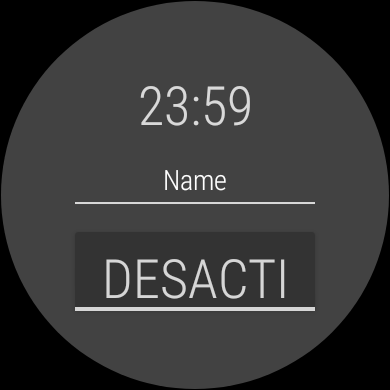
\includegraphics[width=\linewidth]{appActivity.png}
      \caption{\footnotesize Aplicación de gestión}
      \label{fig:uiActivity}
  \end{subfigure}
  \hfill
  \begin{subfigure}[b]{0.4\textwidth}
      \centering
      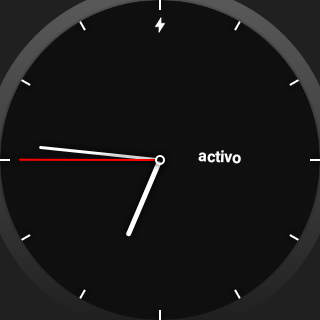
\includegraphics[width=\linewidth]{appWatchface.png}
      \caption{\footnotesize \textit{Watchface}, Interfaz esfera de reloj}
      \label{fig:uiWatchface}
  \end{subfigure}
  \begin{subfigure}[b]{0.4\textwidth}
      \centering
      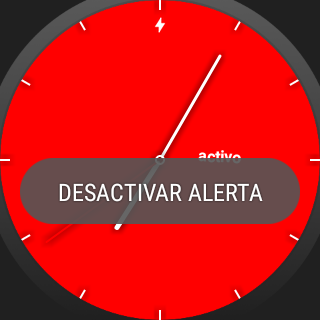
\includegraphics[width=\linewidth]{appAlerta.png}
      \caption{\footnotesize Pantalla de alerta de caída}
      \label{fig:uiAlerta}
  \end{subfigure}
  \hfill
  \begin{subfigure}[b]{0.4\textwidth}
      \centering
      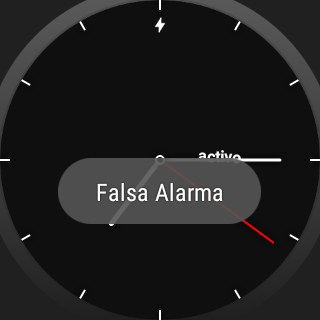
\includegraphics[width=\linewidth]{appAlertaFalsa.png}
      \caption{\footnotesize Pantalla en caso de predetección de caída}
      \label{fig:uiAlertaFalsa}
  \end{subfigure}
  \caption{\footnotesize \label{fig:ifell:UI} Interfaz de usuario de \ifell/}
\end{figure}


La aplicación toma forma de un objeto cotidiano e interactúa con el usuario utilizando un concepto conocido para este: un reloj digital. La única información que se muestra al usuario es la hora (adicionalmente el propio sistema operativo sobreimprime indicaciones de batería baja, ausencia de conexión a internet y existencia de notificaciones de otros servicios y aplicaciones). De esta forma, para el usuario, el dispositivo se convierte en un objeto conocido con un uso muy extendido que de forma adicional a su función tradicional realiza el proceso de detección de caídas.

En esta aplicación se han reducido al máximo las interacciones requeridas por parte del usuario en todo momento, hasta el punto de no requerir ninguna. La aplicación funciona en todo momento como un reloj tradicional mostrando la hora de forma analógica mediante unas manecillas. En el caso de detectarse una caída o evento similar, emitirá de forma automática una serie de avisos visuales, acústicos y hápticos (según las capacidades del dispositivo sobre el que se ejecute) que podrán ser desactivados si se detecta actividad nuevamente. Aunque también existe la posibilidad de desactivarlos tocando la pantalla.

La segunda interfaz que provee la aplicación se encarga de las tareas de administración y configuración. Permite introducir un nombre del usuario y forzar el estado de funcionamiento de los servicios de captura y detección. Si bien ninguno de estos procesos es necesario para el funcionamiento, se ofrece para facilitar la puesta en marcha y prueba del sistema.

\subsubsection{Gestión de alertas}

La aplicación implementada permite alertar tanto desde el propio dispositivo, como mediante mediante una petición sobre HTTP hacia la API \texttt{alertaCaida} que se ejecuta en el servidor. De manera local la aplicación alerta visualmente mediante un mensaje sobreimpreso en la pantalla, y en los dispositivos que lo admitan una vibración rítmica y un pitido. En caso de un falso evento o de querer interrumpir la alarma se puede desactivar tocando una vez la pantalla. 

Hay que recalcar que dada la estructura de módulos con estructura emisor-consumidor asíncronos, el servicio de detección de caídas no deja de funcionar en ningún momento, y podría lanzar un segundo evento de caída incluso durante la alarma del primero. El modelo es capaz de detectar una nueva caída 

El dispositivo utilizado para el estudio no dispone de altavoz para emitir alertas acústicas, pero la vibración es más que suficiente para alertar al usuario de la detección de la caída y de ser necesario desactivar la alarma.




\todo{Faltaría una sección de comunicación con el servidor}


\section{Elección de parámetros y generación del modelo final}

Una vez confirmado el funcionamiento del algoritmo sobre la base de datos \ifell/ el último paso es generar el modelo a embarcar en la aplicación a probar. Durante las etapas previas hemos adelantado ya la elección de centrar la ventana de salida de la red en el instante de detección del modelo de Bourke $t_0$. Por tanto trabajaremos con los siguientes casos:
  \begin{itemize}
    \item \textit{RNN-reconstrucción} Dos ventanas: $W_i$ la ventana de entrada, y $W_o$ la ventana de salida. En este caso ambas coinciden y empiezan en $W_i=W_o=X[t_0-50, t_0+50]$, y contienen 100 muestras o 4 segundos.
    \item \textit{RNN-predicción} De nuevo dos ventanas $W_i$ y $W_o$ de entrada y salida pero esta vez no solapadas. La ventana de entrada con el fragmento de señal $W_i=X[t_0-125,t_0-25]$ y la ventana de salida, con el fragmento a predecir de únicamente dos segundos (50 muestras) que incluye las muestras $W_o=X[t_0-25, t_0+25]$.
  \end{itemize}

  Estas ventanas y el centrarlas en el momento del impacto ya lo avanzamos en el apartado \ref{subsub:ifell:windowing} sin embargo en la realización probamos varias configuraciones con retrasos del punto de impacto (ditancia desde el inicio de la ventana de salida $W_o$ hasta el instante $t_0$) diferentes. 

  El siguiente parámetro a determinar es el tamaño del espacio intermedio, o el número de atributos que genera el codificador e interpreta el decodificador. Veremos el impacto que tiene en la calidad del estimador y tiempo de respuesta de este factor antes de fijar un valor.

  Con estos parámetros del modelo fijados nos queda realizar un último ejercicio para elegir la arquitectura. Decidiremos tanto el número de celdas por capa como si optamos por un modelo de predicción o de reconstrucción de la señal analizando los resultados de los mejores modelos y teniendo en consideración la latencia de los modelos. No abordaremos por contra los efectos de las diferentes técnicas de optomización aplicadas ya que las evaluaremos debidamente en el siguiente capítulo.

  Con la arquitectura fijada y los parámetros del modelo definidos entrenaremos el modelo final de \ifell/ usando el conjunto de datos obtenido gracias a \accelcapture/. Definiremos los parámetros finales del modelo de Bourke a utilizar mediante este mismo conjunto y evaluaremos la calidad del modelo sobre esta base de datos.

\subsection{Evaluación del algoritmo sobre \ifell/}

Para estudiar impacto del número de atributos, arquitectura de red y posición de la ventana de salida, evaluamos diferentes combinaciones sobre el subconjunto de datos de test. Como ya mencionamos este subconjunto mantiene la proporción original de caídas y actividades del conjunto original, y por tanto la estadística debería mantenerse. 

Al usar el error RMSE entre la salida del modelo y la señal enventanada $W_o$, podemos realizar el mismo ejercicio que al analizar el conjunto de datos \ifell/ de analizar la distribución de los errores de predicción de los modelos. Podemos comparar los resultados con la distribución de las cotas superiores que hemos estudiado en la sección \ref{sub:imp:model:algoritmo}. El efecto de los modelos debería separar las funciones de distribución del RMSE de las actividades del error de las caídas con respecto a la distribución obtenida para los modelos de Bourke.

\figura{HistoRMSE}{fig:ifell:rmse:histograma}{Histograma del error RMSE de actividades y caídas}


Si comparamos los histogramas obtenidos (como por ejemplo el de la figura \ref{fig:ifell:rmse:histograma}) con los obtenidos previamente en el análisis del modelo de Bourke (\ref{fig:bourke:hist}) observamos como el resultado se asemeja más al obtenido para el análisis de las cotas \textit{ULF} de Bourke, aunque con una separación ligeramente mayor, especialmente por la mayor concentración de actividades cerca del 0. Este es un indicador esperanzador para los resultados finales pues muestra que el modelo ha conseguido aumentar la distancia entre las actividades y caídas con respecto al clasificador \textit{BourkeU}.

Finalmente analizamos el impacto del tamaño del modelo, posición de la ventana $W_o$ respecto al instante de detección $t_0$, de los modelos de predicción y reconstrucción y añadimos una nueva variante: la sensibilidad objetivo mediante la variación de la cota de decisión del error RMSE. Si observamos las figura \ref{fig:ifell:confmats}, que contiene dos ejemplos de matriz de matrices.Los modelos usados son las variaciones de los modelos de tres capas GRU de 350 unidades y 50 atributos, tanto para reconstrucción como para predicción. Hemos elegido estas dos muestras por ser representativas del comportamiento observado en cada familia y para poder comparar ambas a su vez en igualdad de tamaño de los modelos.


\begin{sidewaysfigure}[!ht]
  \centering
  \begin{subfigure}[b]{0.45\textwidth}
      \centering
      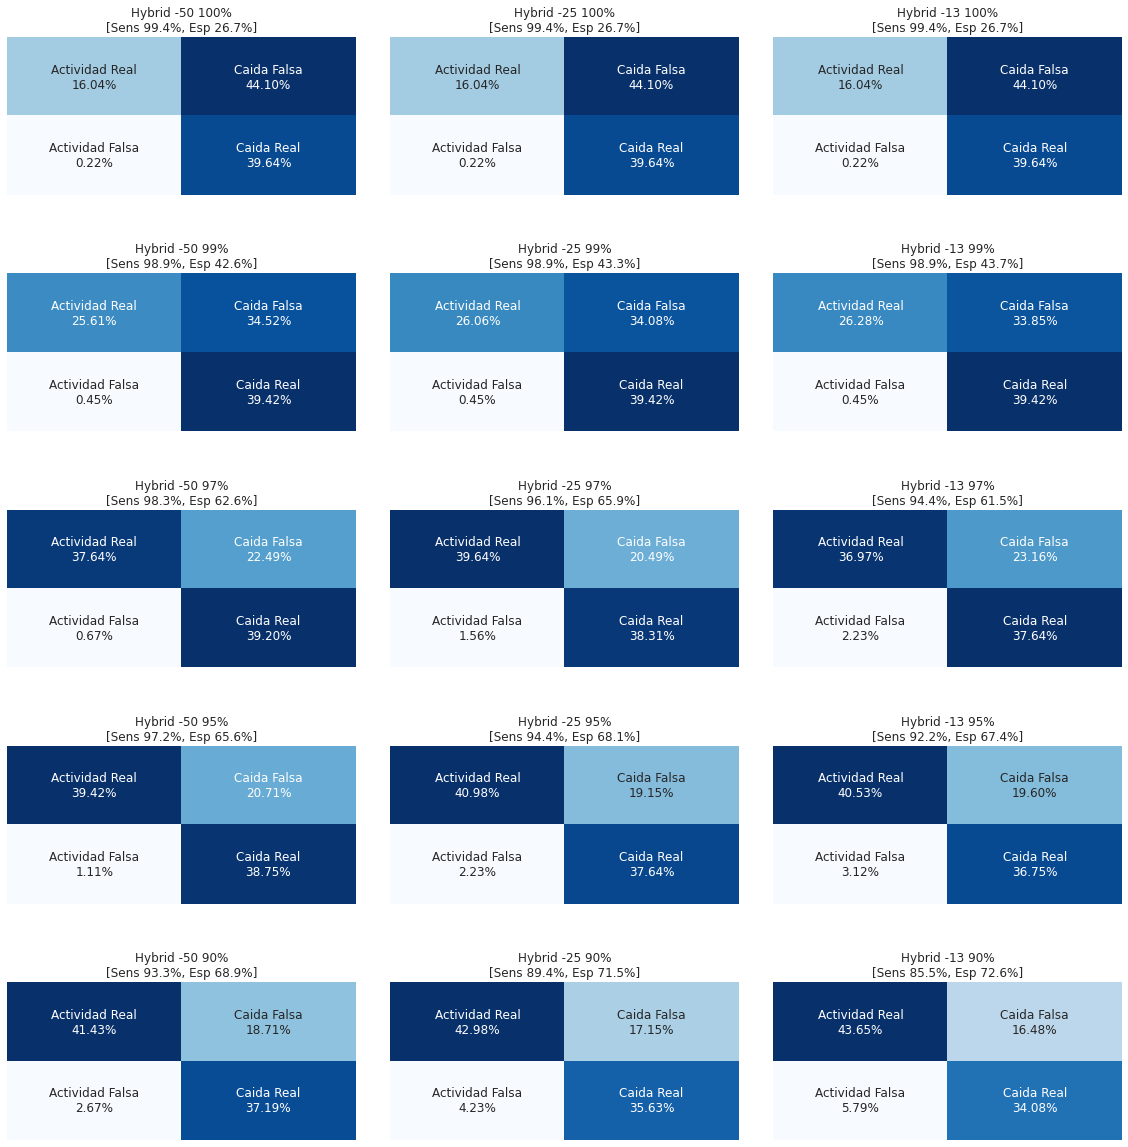
\includegraphics[width=\linewidth]{ConfMatrixRecon.png}
      \caption{\footnotesize \label{fig:ifell:confmat:recon}Matrices de confusión para un modelo de reconstrucción}
  \end{subfigure}
  \hfill
  \begin{subfigure}[b]{0.45\textwidth}
      \centering
      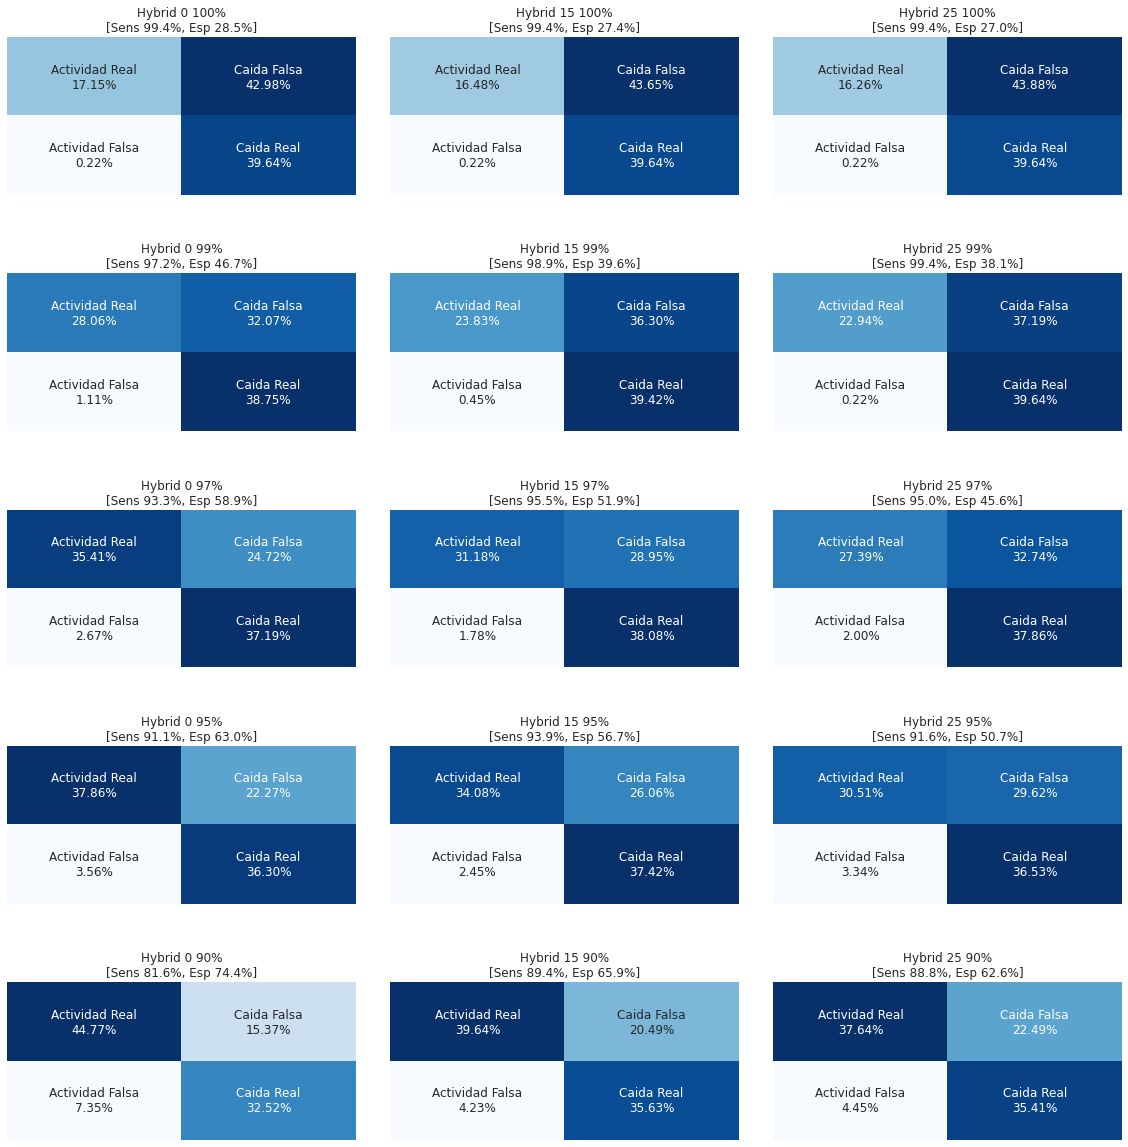
\includegraphics[width=\linewidth]{ConfMatrixPred.png}
      \caption{\footnotesize \label{fig:ifell:confmat:pred}Matrices de confusión para un modelo de predicción}
  \end{subfigure}
  \caption{\label{fig:ifell:confmats}Ejemplos de matrices de confusión según sensibilidad deseada y posición de la ventana}
\end{sidewaysfigure}

En estas tablas usamos la distancia en muestras \textit{desde el final de la ventana $W_i$} hasta el instante $t_0$ como índice para definir la posición de las ventanas respecto al instante de pre-detección. Así en los modelos de reconstrucción estos desplazamientos han de ser siempre negativos, mientras que para los modelos de predicción han de ser positivos. Por ejemplo, el valor -50 se correspondería al centro de la ventana $W_i$ en un modelo de reconstrucción (Si $W_i=W_o$ contiene las muestras entre 1 y 100, desplazarnos -50 muestas significa situar $t_0$ en la muestra $t_0=100-50 = 50$ de ambas ventanas) o para un caso de predicción, el valor 13 indicaría que la ventana de salida empieza 13 muestras antes del punto de impacto (en este caso $t_0 = 100 + 13$ con $W_i$ las muestras de 1 a 100 y $W_o$ las muestras a predecir entre 101 y 150).

Para mejor ilustrar y favorecer la toma de decisiones decidimos valorar cada posible modelo con una nota basada en la media ponderada entre sensibilidad y especificidad tal que $Nota=\frac{2Sensibilidad+Especificidad}{3}$ dándole efectivamente el doble de peso a la métrica de sensibilidad sobre especificidad en el cómputo. Los resultados para las matrices de la figura \ref{fig:ifell:confmats} quedarían como se observa en la \autoref{tab:nota:estimadores}.

\tablas{tab:nota:estimadores}{Nota de los estimadores}{lrrrrrr}{ 
                         & \multicolumn{3}{c}{\textit{RNN-Reconstrucción}}   & \multicolumn{3}{c}{\textit{RNN-Predicción}}   \\ \cmidrule{2-4}\cmidrule{5-7}   
Sensibilidad Objetivo    & $\Delta t=-50$ & $\Delta t=-25$ & $\Delta t=-13$ & $\Delta t=0$ & $\Delta t=15$ & $\Delta t=25$ \\ \midline
100\%                   & 751 & 751 & 751 & 754 & 754 & 752 \\
99\%                    & 801 & 803 & 805 & 803 & 791 & 789 \\
97\%                    & 864 & 860 & 834 & 818 & 809 & 785 \\
95\%                    & 866 & 856 & 839 & 817 & 815 & 779 \\
90\%                    & 851 & 834 & 812 & 792 & 815 & 800 \\
}{3}

Con este varemos, a igualdad de tamaño del modelo, el de reconstrucción muestra mejor capacidad de detección, especialmente si posicionamos $t_0$ en el centro de la ventana, aunque dados los resultados si se retrasa a 25 muestras del final de la ventana, posiblemente el mejor caso estaría en una posición intermedia entre ambas. Si bien este resultado es consistente a lo largo de todos los modelos de reconstrucción, encontrar una tendencia similar en los modelos de predicción es más complejo. En este ejemplo se observa como si buscamos alta sensibilidad cuanto menos retrasemos $t_0$ mejor es el estimador, pero si buscamos un mejor estimado según la nota en general se consigue con valores $\Delta t \approxeq 15$. 

\tablas{tab:nota:mejor:estimador}{Mejor estimador de cada modelo} {lcccc}{
  \textit{Modelo}     & \textit{Nota} & $\Delta t$ & \textit{Sensibilidad} (\%) & \textit{Especificidad} (\%) \\ \midrule
RNN-R(350)[50] & 851 & -25 & 96,6 & 62,2 \\
RNN-P(350)[50] &     &     &      &      \\
RNN-R(350)[30] & 847 & -25 & 98,0 & 58,1 \\
RNN-P(350)[30] & 828 & 15  & 93,9 & 60,7 \\
RNN-R(175)[50] & 866 & -25 & 97,2 & 65,6 \\
RNN-P(175)[50] & 818 & 0   & 93,3 & 58,9 \\
RNN-R(175)[30] & 862 & -25 & 98,3 & 62,2 \\
RNN-P(175)[30] & 822 & 15  & 94,4 & 63,0 \\
}{2}

De los resultados expuestos en la \autoref{tab:nota:mejor:estimador} se aprecia que los modelos grandes no son mejores detectores que los de tamaño menor. Es consistente la superioridad de los detectores por reconstrucción sobre los de predicción, así como el impacto de reducir el número de atributos ofreciendo resultados ligeramente peores, ( aunque mejores en promedio, los estimadores resultantes tienen peor nota superior que sus equivalente de 50 atributos). En general apreciamos una mayor variabilidad en los resultados de los clasificadores por predicción, por ejemplo es dificil elegir una posición ideal para la ventana respecto a $t_0$ y la reducción de número de atributos del codificador/decodificador tiene un impacto aleatorio, a veces mejora y a veces peora el rendimiento.



\subsection{Entrenamiento del modelo RNN final}

Entrenaremos dos modelos finales para poder confrontarlos y el elegir el mejor estimador de los dos. Los dos modelos siguen la mencionada arquitectura codificador/decodificador, con simetría entre ambos componentes. Cada uno está conformado por 3 capas GRU de 175 unidades cada una. El codificador genera un vector de 50 atributos a partir del estado interno de una cuarta capa GRU de 50 unidades, idénticas estructuras a las mostradas en la \autoref{fig:rnnFinal} pero de 175 unidades. Generamos ambas variantes a las que designaremos por los nombres \textit{IFELL-P(175)[50]} para el modelo de predicción e \textit{IFELL-R(175)[50]} para el modelo de reconstrucción para diferenciarlos de los modelos de idéntica arquitectura entrenados con la abse de datos \sisfall/.

De manera similar a como se realizó para los modelos entrenados con sisfall separamos el 20\% del conjunto de datos obtenido por \accelcapture/ para la validación del modelo y utilizaremos el restante 80\% para su entrenamiento. Los parámetros de entrenamiento se mantienen: Entrenaremos máximo 200 iteraciones usando un mecanismo de parada anticipada si durante 5 iteraciones no mejora el aprendizaje de la red. Usaremos Adam como optimizador, con una tasa de aprendizaje que de nuevo es decreciente de forma no lineal para favorecer la velocidad del entrenamiento sin penalizar el ajuste fino de la red hacia en las últimas etapas de entrenamiento. 

\begin{figure}[htb!]
  \centering
  \begin{subfigure}[b]{0.47\textwidth}
      \centering
      \pincludegraphics[1.0]{ADATA_RECON_TRAIN}
      \caption{\footnotesize \label{fig:ifell:adata:recon:train} Evolución RMSE durante entrenamiento del modelo de reconstrucción}
  \end{subfigure}
  \centering
  \hfill
  \begin{subfigure}[b]{0.47\textwidth}
      \centering
      \pincludegraphics[1.0]{ADATA_PRED_TRAIN}
      \caption{\footnotesize \label{fig:ifell:adata:pred:train} Evolución RMSE durante entrenamiento del modelo de predicción}
  \end{subfigure}

  \begin{subfigure}[b]{0.47\textwidth}
      \centering
      \pincludegraphics[1.0]{ADATA_RECON_PRUNE}
      \caption{\footnotesize \label{fig:ifell:adata:recon:prune} Evolución RMSE durante el cribado del modelo de predicción}
  \end{subfigure}
  \begin{subfigure}[b]{0.47\textwidth}
      \centering
      \pincludegraphics[1.0]{ADATA_PRED_PRUNE}
      \caption{\footnotesize \label{fig:ifell:adata:pred:prune} Evolución RMSE durante el cribado del modelo de predicción}
  \end{subfigure}
  \caption{\label{fig:ifell:adata:training} Gráficas del error RMSE durante el entrenamiento y pruning de los modelos IFELL-R(175)[50] e IFELL-P(175)[50]}
\end{figure}
De idéntica manera a como se hizo con los modelos usados para probar el algoritmo, optimizaremos mediante pruning cribando el 50\% de los pesos y posteriormente discretizándolos. En la figura \ref{fig:ifell:adata:training} se muestra la evolución del RMSE de los modelos durante el entrenamiento y pruning. El modelo de predicción está claramente sobreajustando al conjunto de entrenamiento, incluso tras el cribado, por lo que esperamos un modelo con menor capacidad de generalizar.

Finalmente en el siguiente capítulo probamos el algoritmo usando los modelos \textit{IFELL-R(175)[50]} e \textit{IFELL-P(175)[50]} sobre la base de datos de \sisfall/. Los resultados obtenidos nos permiten evaluar el rendimiento del algoritmo por si mismo así como compararlo con los modelos \textit{RNN-R(175)[50]} y \textit{RNN-P(175)[50]} que se entrenaron y evaluaron con \sisfall/. Como parámetros para el modelo de Bourke decidimos tomar una cota superior de 5\g/. Esta cota está por encima del mínimo pico detectado para caídas, pero lo tomamos por ser más selectivo con las actividades ordinarias mientras que penaliza mínimamente la sensibilidad (-0,6\%).

